\documentclass[a4paper,11.5pt, table]{article}

%%%%%% Basic packages begin %%%%%%
\usepackage[
	textwidth  = 160mm, 
	textheight = 230mm, 
	top        = 25mm, 
	bottom     = 30mm
]{geometry}
\usepackage[normalem]{ulem}
\usepackage[utf8]{inputenc}
\usepackage[T1]{fontenc}
\PassOptionsToPackage{defaults=hu-min}{magyar.ldf}
\usepackage[magyar]{babel}
%%%%%%% Basic packages end %%%%%%%

%%%%%% Packages required for this document begin %%%%%%
\usepackage{
	amsmath,   % Math mode
	amsthm,    % "note" environment
	amsfonts,  % "\mathbb{}" command
	paralist,  % "compactitem" and "compactenum" environment
	multirow,  % "\multirow{}{}" command
	float,     % "H" float specifier
	tikz,      % Basepackage for nearly all figures
	listings,  % Used for code snippets
	etaremune, % Reverse compactenum
%	graphicx   % For including images
	enumitem   %for alphabetical enumeration
}
\usepackage[unicode]{hyperref} % Clickable links
%%%%%%% Packages required for this document end %%%%%%%

%%%%%% TikZ options start %%%%%%
\usetikzlibrary{
	positioning, % Contains positioning utilities, such as "below = of" 
	calc,        % Adding coordinates
	math         % Needed for global variables
}

\tikzstyle{NodeBase} = [
	rectangle,
	text centered,
	draw = black
]

\definecolor{DefaultObjectColor}{gray}{0.9} % This is the default color of object in the TikZ pictures

\tikzstyle{arrow} = [
	thick,
	->,
	>=stealth
]
%%%%%%% TikZ options end %%%%%%%

%%%%%% lstlistings envvironment options start %%%%%%

\lstdefinestyle{customc}{ % C/C++ code snippet style
	belowcaptionskip = 1\baselineskip,
	breaklines       = true,
	frame            = L, % Double line on the left
	language         = C++,
	showstringspaces = false,
	basicstyle       = \ttfamily,
	keywordstyle     = \bfseries\color{green!40!black},
	stringstyle      = \color{orange},
	emphstyle        = \color{blue}, % Defined below
	tabsize          = 4,
	columns          = fullflexible,
}

\lstset{
	escapechar = @,
	style      = customc, % Default code snippet style
	%NOTE In order to use special characters in code snippets, one has to manually define them.
	literate   = {á}{{\'a}}1 {é}{{\'e}}1 {í}{{\'i}}1 {ó}{{\'o}}1 {ú}{{\'u}}1	{Á}{{\'A}}1 {É}{{\'E}}1 {Í}{{\'I}}1 {Ó}{{\'O}}1 {Ú}{{\'U}}1	{ö}{{\"o}}1 {ü}{{\"u}}1 {Ö}{{\"O}}1 {Ü}{{\"U}}1
	{ű}{{\H{u}}}1 {Ű}{{\H{U}}}1 {ő}{{\H{o}}}1 {Ő}{{\H{O}}}1
	{€}{{\euro}}1 {£}{{\pounds}}1 {~}{$\sim$}{1}	
}

%%%%%%% lstlistings envvironment options end %%%%%%%

%%%%%%%% Compilation error fix begin %%%%%%%%
\makeatletter
\expandafter\let\csname active@char\string?\endcsname\relax
\expandafter\let\csname active@char\string!\endcsname\relax
\expandafter\let\csname active@char\string:\endcsname\relax

\initiate@active@char{?}
\initiate@active@char{!}
\initiate@active@char{:}
\makeatletter
%%%%%%%%% Compilation error fix end %%%%%%%%%

\setlength{\parindent}{0mm}
\setlength{\parskip}{1em}
\setcounter{section}{0}

\begin{document}
	\begin{center}
		{\LARGE Adatbázisok II.}
		\smallskip
		
		{\large 2. ZH elméleti része}
	\end{center}
	A jegyzetet \textsc{Csonka} Szilvia írta. A jegyzet első számú forrása a gyakorlat.\\
	
	
	
	
	
	\textbf{Információk}
	\begin{compactitem}
		\item pótZH: vizsgaidőszak 1. hetében.
		\item A ZH $\frac{1}{4}$ 9-kor kezdődik.
	\end{compactitem}
	
	\section{Rész}
	
	\textbf{Források}
	\begin{compactitem}
	\item A feladatsor és további elméleti részek \textsc{Nikovits} Tibor honlapján: \url{http://people.inf.elte.hu/nikovits/AB2/ab2_feladat9.txt}.
	
	\item További kapcsolódó források a gyakorlatvezető honlapjáról:
	\begin{compactitem}
		\item UW\_redo\_naplo.doc
		\item UW\_undo\_naplo.doc
		\item UW\_undo\_redo\_naplo.doc
	\end{compactitem}
	
	\item Az előadás honlapján található (\url{http://people.inf.elte.hu/kiss/15ab2/13ab2osz.htm}) \textit{naplo.ppt} egyes diái (a 8., 9., 10. előadás anyagai között megtalálható) szintén segítségül szolgálnak az alábbi feladatok megoldásának megértéséhez. 
	\end{compactitem}
	
	
	\textbf{8.1.1 Feladat} (könyv 463. old.)
	
	Tegyük fel, hogy az adatbázisra vonatkozó konzisztenciamegszorítás: 0 <= A <= B. \\
	Állapítsuk meg, hogy a következő tranzakció megőrzik-e az adatbázis konzisztenciáját.\\
	\textbf{\textit{T1:}} $ A := A + B; B := A + B;$
	\begin{itemize}
		\item \textit{Megjegyzés:} itt valójában $B := A + 2B$ fog végrehajtódni, ugyanis az értékadásokat szekvenciálisan, egymás után fogjuk végrehajtani. 
		
		\item \textit{Megoldás:}\\
		\begin{lstlisting}
	INPUT(A)					//A-t beolvassuk a memóriapufferbe a lemezről
	INPUT(B)					//B-t is
	READ(A, t)			//a memóriából a t lokális változóba másoljuk A-t
	READ(B, s)			//B-t pedig s-be
	t := t + s			//végrehajtjuk a kért értékadások közül az elsőt
	WRITE(A, t)		//az eredményt a memóriapufferbe írjuk 
	s := s + t			//végrehajtjuk a második értékadást is
	WRITE(B, s)		//ezt is a memóriába írjuk
	OUTPUT(A)				//a memóriából a lemezre mentjük A eredményét 
	OUTPUT(B)				//B-ét is
		\end{lstlisting}
		
		\item \textit{Mejegyzés:} itt nem kérdezték a naplózást, így azt ebben a feladatban nem kell részleteznünk.
	\end{itemize}

	\textbf{8.2.4 Feladat}(könyv 476. old.)
	
	A következő naplóbejegyzés-sorozat a T és U két tranzakcióra vonatkozik:
	\begin{lstlisting}
	<start T> 
	<T, A, 10> 
	<start U> 
	<U, B, 20> 
	<T, C, 30> 
	<U, D, 40>
	<T, A, 11>
	<U, B, 21>  
	<COMMIT U>
	<T, E, 50> 
	<COMMIT T>
	\end{lstlisting}
	Adjuk meg a helyreállítás-kezelő tevékenységeit, ha az utolsó lemezre került naplóbejegyzés:
	\begin{enumerate}[label=\alph*)]
		\item <start U> 
		\item <COMMIT U>
		\item <T, E, 50>
		\item <COMMIT T>
	\end{enumerate}
	
	\begin{itemize}
		\item \textbf{\textit{Megoldás UNDO helyreállítás \textit{(lásd. naplo.ppt 54. dia)} esetén:}}
			\begin{enumerate}[label=\alph*)]
				
				
				\item Az adatvesztéssel járó hiba bekövetkeztéig a következők futottak le:
				\begin{lstlisting}
	<start T> 
	<T, A, 10> 
	<start U> 
				\end{lstlisting}
				\textit{Megoldás:}
				\begin{lstlisting}
	WRITE(A, 10)	//Visszaállítjuk A T tranzakció lefutása előtti állapotát.
	OUTPUT(A)				//Lemezre írjuk A helyreállított változatát.
	<T, ABORT>			//Naplózzuk, hogy T tranzakció eredményét visszaállítottuk.
				  //Azaz helyreállítottuk, a nem teljesen lefutott tranzakció
				  // okozta nem konzisztesn állapotot, hogy ismét konzisztens
				  // legyen az adatbázis.
	FLUSH LOG			   //Naplózást is lementjük.
				\end{lstlisting}
				
				
				\item Az adatvesztéssel járó hiba bekövetkeztéig a következők futottak le:
				\begin{lstlisting}
	<start T> 
	<T, A, 10> 
	<start U> 
	<U, B, 20> 
	<T, C, 30> 
	<U, D, 40>
	<T, A, 11>
	<U, B, 21>  
	<COMMIT U>
				\end{lstlisting}
				\textit{Megoldás:}
				\begin{lstlisting}
	WRITE(A, 11)
	OUTPUT(A)
	WRITE(C, 30)
	OUTPUT(C)
	WRITE(A, 10)
	OUTPUT(A)
	<T, ABORT> //Naplóbejegyzés: helyreállítottuk A állapotát a T előttire
	FLUSH LOG		//Lementjük a fenti naplóbejegyzést is.
				\end{lstlisting}
				\textit{Megjegyzés:} Visszaállítjuk a dolgokat a napló végétől az eleje felé haladva. Az \textit{U} tranzakció által végrehajtott módosításokat nem kell helyreállítanunk, ugyanis a hiba előtt ez már sikeresen lefutott és le is lett mentve (\textit{COMMIT}) az eredménye, tehát nem zavar bele az adatbázis konzisztenciájába.
				
				
				\item (Gyakorlaton nem volt.)
				
				\item Minden le lett mentve az adatvesztéssel járó hiba előtt, tehát nem szükséges semmit sem helyreállítani. :)				
			\end{enumerate}
		\item \textbf{\textit{Megoldás REDO helyreállítás (lásd. naplo.ppt 78. dia) esetén:}}\\
		\textit{Megjegyzés:} a dián a végéről lemaradt a "FLUSH LOG".
		
		\begin{enumerate}[label=\alph*)]
			\item (Nem volt gyakorlaton.)
			\item Az adatvesztéssel járó hiba bekövetkeztéig a következők futottak le:
			\begin{lstlisting}
	<start T> 
	<T, A, 10> 
	<start U> 
	<U, B, 20> 
	<T, C, 30> 
	<U, D, 40>
	<T, A, 11>
	<U, B, 21>  
	<COMMIT U>
			\end{lstlisting}
			\textit{Megoldás:}
			\begin{lstlisting}
	WRITE(B, 20)
	OUTPUT(B)
	WRITE(D, 40)
	OUTPUT(D)
	WRITE(B, 21)
	OUTPUT(B)
	FLUSH LOG
			\end{lstlisting}
			\textit{Megjegyzés:}\\
			\textit{REDO} esetén azokat az adatokat állítjuk helyre a tranzakció lefutása utáni állapotukra, amelyekre volt \textit{COMMIT}, azaz lefutottak, csak eredményük nem került egészében mentésre (mivel eközben következett be a hiba), azaz nem volt \textit{END}. Így mivel \textit{U} tranzakcióra volt \textit{COMMIT}, de \textit{END} nem, ezért a fenti példában ennek az eredményét állítottuk helyre. \textit{T}-vel nem foglalkozunk, hiszen arra \textit{COMMIT} sem volt, azaz be sem fejeződött, így nincs lenaplózva és nem is tudhatjuk az összes adatváltoztatásának következményét (azaz ha helyreállítanánk a naplóban szereplő eddigi adatváltoztatásait, nem konzisztens állapotú adatbázist kapnánk).
		\end{enumerate}
		
	\end{itemize}

	\textbf{Az Oracle naplózása}
	\begin{itemize}
		\item Az Oracle valójában \textit{REDO} naplózást használ. Így elég csak az utasítást lementenie egy update-ről.
		
		\item Az \textit{UNDO} naplózásra külön \textit{UNDO táblateret} használ, mivel ez nagyon memóriaigényes, hiszen ekkor az összes olyan táblaelem korábbi értékét le kell menteni, amelyet az adott update megváltoztatott, azaz előfordulhat, hogy komplett táblákat kell eltárolni. Ezen mentések felhasználásával tudja megoldani az Oracle, hogy amennyiben egyszerre többen használnak egy táblát, akkor a használat kezdeti pillanatbeli állapotát bocsájtja a felhasználó rendelkezésére a táblának.
	\end{itemize}

\newpage

	\section{Rész}

	\textbf{Források}
	\begin{compactitem}
		\item Az előadás diái közül a \textit{konkurencia.ppt}, mely a 10., 11., 12. előadás anyagánál megtalálható az előadó honlapján: \url{http://people.inf.elte.hu/kiss/15ab2/13ab2osz.htm}
		 \item A tankönyv ütemezésekre vonatkozó része a gyakorlat honlapján: \url{http://people.inf.elte.hu/nikovits/AB2/} \textit{UW\_utemezesek.doc}.
		\item A feladat és további elméleti részek \textsc{Nikovits} Tibor honlapján: \url{http://people.inf.elte.hu/nikovits/AB2/ab2_feladat10.txt}
	\end{compactitem}

	\textbf{Soros ütemezések} \textit{(konkurencia.ppt 6.dia)}
	\begin{compactitem}
		\item "Két tranzakciónak két soros ütemezése van, az egyikben T$_{1}$ megelőzi T$_{2}$‑t, a másikban T$_{2}$ előzi meg T$_{1}$-et."
		
		\item Probléma: több tranzakciót egyszerre kéne végrehajtani olyan sorrendben, amely olyan eredményt kapjunk, mintha sorosan hajtottuk volna őket végre.
		
		\item Mindegy, hogy T$_{1}$ és T$_{2}$ egyszerre végrehajtott tranzakciók közül melyik hajtódik végre először, a lényeg a konzisztencia megőrzése.		
	\end{compactitem}

	\textbf{Ütemezés} \textit{(konkurencia.ppt 3. dia)}
	\begin{compactitem}
		\item "Az ütemezés (schedule) egy vagy több tranzakció által végrehajtott lényeges műveletek időrendben vett sorozata, amelyben az egy tranzakcióhoz tartozó műveletek sorrendje megegyezik a tranzakcióban megadott sorrenddel"
		
		\item Szemléletesen:
		\begin{compactitem}
			\item Képzeljük el, hogy egy kereszteződésben több különböző út találkozik, melyekről egyszerre érkeznek autók melyek mind egy adott útra akarnak besorolni, melyről nem jön senki.
			\item Az ütemező egy sorrendet állít fel, mint egy forgalmat irányító rendőr.
			\item Elvárások:
			\begin{compactitem}
				\item Az azonos útról érkező autók sorrendje ne változzon!
				\item Azaz egy tranzakció műveleteit adott sorrendben kell elvégezni, de attól még más tranzakciók műveleteit csinálhatjuk közben.
			{compactitem}
			\begin{figure}[h]
				\centering
				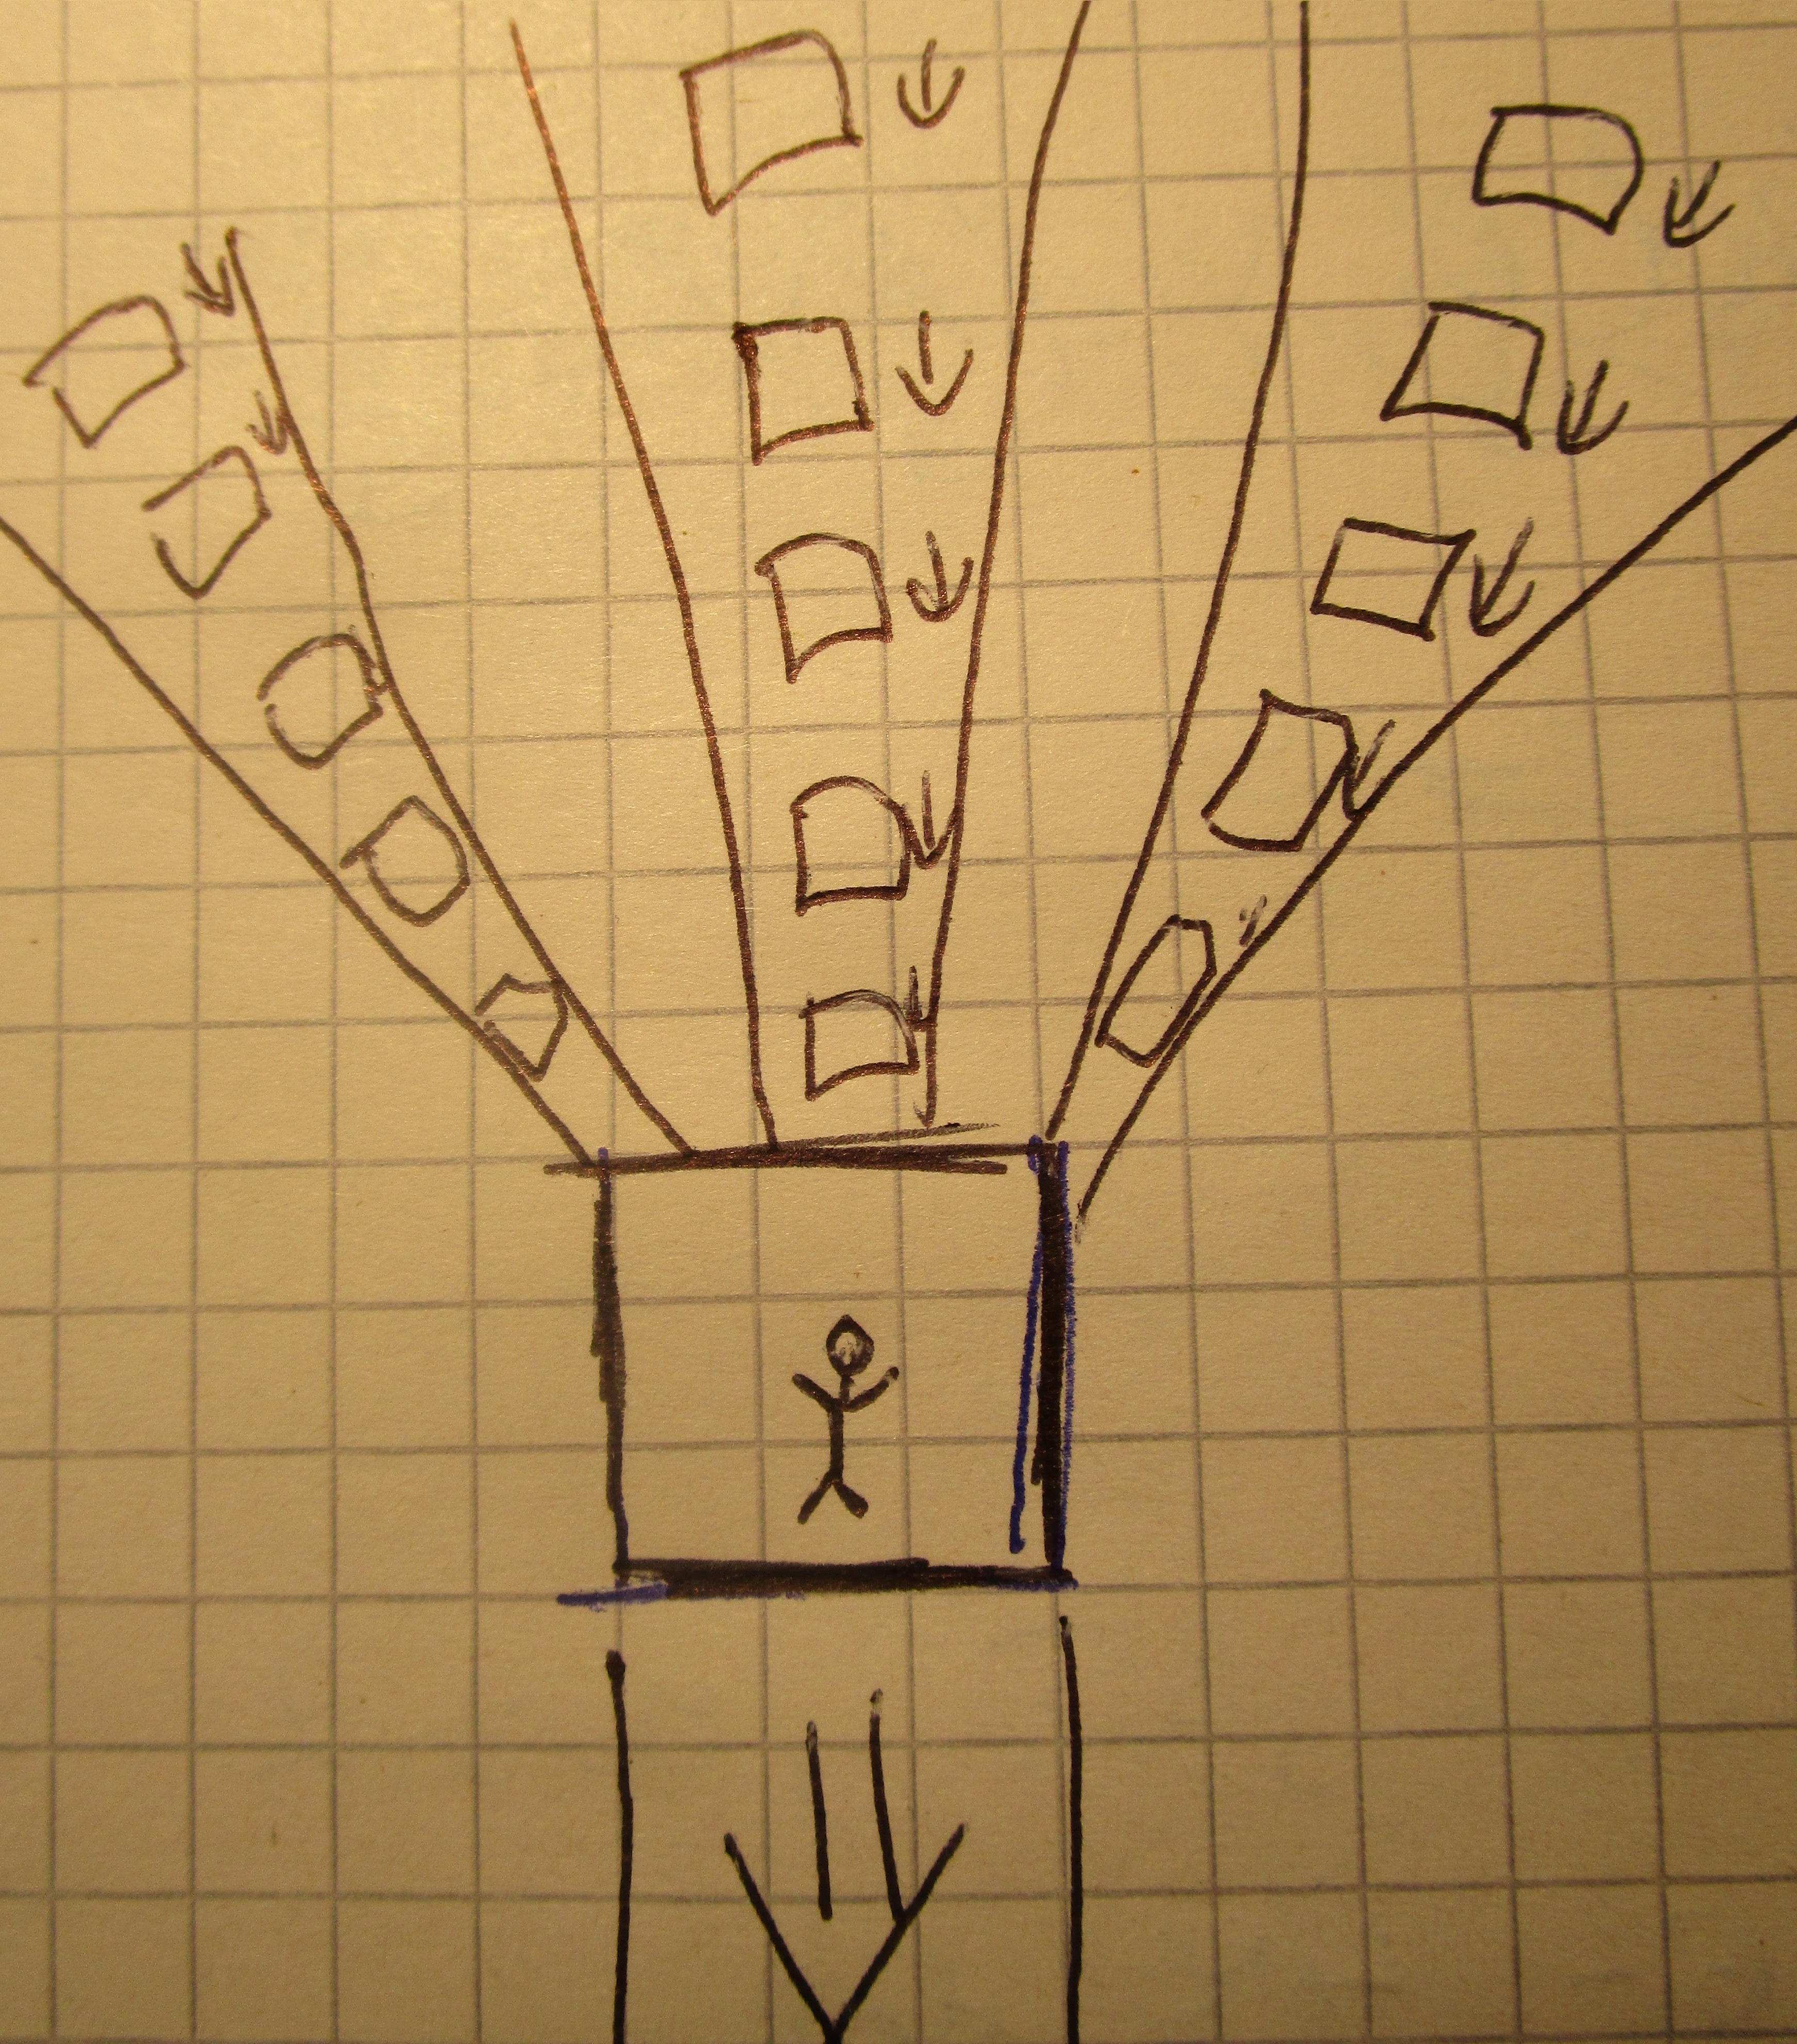
\includegraphics[height = 5cm]{abra.jpg}
			\end{figure}
			\end{compactitem}
		\end{compactitem}
	\end{compactitem}
	

	\textbf{9.1.2 Feladat}
	
	Adott az alábbi három tranzakció:
	\begin{lstlisting}
	T1: READ(X,t); t:=t+100; WRITE(X,t);
	T2: READ(X,t); t:=t*2; WRITE(X,t);
	T3: READ(X,t); t:=t+10; WRITE(X,t);
	\end{lstlisting}
	\begin{enumerate}[label=\alph*)]
		\item Hányféle különböző ütemezése van a fenti 3 tranzakciónak?  
		\begin{compactitem}
			\item Ekkor nem törődünk azzal, hogy az egyes műveletek mely tranzakcióhoz tartoznak, de azt szem előtt tartjuk, hogy bár nem sorosan hajtjuk őket végre, de az eredménynek olyannak kell lennie, mintha ezt tettük volna.
			
			\item Összesen 9 műveletet szeretnénk végrehajtani, ha semmit sem veszünk figyelembe, ezt $9!$ féle képpen tehetjük meg.
			
			\item Ekkor amit még nem vettünk figyelembe: egy tranzakcióhoz tartozó lépések egymáshoz képesti sorrendje ne változzon.
			\begin{compactitem}
				\item Ezeknek egymáshoz viszonyított sorrendjét $3!$ féle képpen cserélhetjük fel.
				\item A fenti $9!$-ban ez az egy tranzakcióhoz tartozó műveletek $3!$ féle cseréje is benne van. 
				\item Tehát az egy tranzakcióhoz tartozó műveletek egymáshoz való sorrendjének változtatásával létrehozott verziók számával leosztva a $9!$-t kapjuk a kért darabszámot. 
			\end{compactitem}
			
			\item Tehát a megoldás: 
			\begin{center}
				 \LARGE $\frac{9!}{3!  3!  3!}$
			\end{center}
		\end{compactitem}
		
		\item Hányféle soros ütemezése van a fenti 3 tranzakciónak?
		\begin{compactitem}
			\item Soros ütemezés esetén a 3 tranzakció lépéseit nem cserélgetjük, hanem először végrehajtjuk az egyik tranzakció összes lépését, majd ha azzal mind megvagyunk, akkor veszünk egy másikat, és azzal is így tovább...
			
			\item Azaz először 3 tranzakció közül végrehajtunk 1-et, majd a maradék 2 közül választunk 1-et, majd megcsináljuk az utolsót is.
			
			\item Ez így összesen: \textbf{$3$! féle soros ütemezés}. 
		\end{compactitem}
	\end{enumerate}

	\textbf{9.2.1 Feladat}

\end{document}